% Standalone Overleaf document. Compile this file with pdfLaTeX.
% Revised from the researcher-supplied September 23 source. This edited edition is not generated from the older Markdown; do not overwrite it with the legacy generator.
\documentclass[11pt,letterpaper]{article}
\usepackage[T1]{fontenc}
\usepackage[utf8]{inputenc}
\usepackage{lmodern,microtype}
\usepackage[margin=0.75in,headheight=16pt]{geometry}
\usepackage{xcolor}
\definecolor{Gold}{HTML}{FFC904}
\definecolor{Ink}{HTML}{171717}
\definecolor{Gray}{HTML}{626262}
\definecolor{ActionInk}{HTML}{665117}
\definecolor{NoteFill}{HTML}{FFF8DD}
\usepackage{titlesec,enumitem,tabularx,fancyhdr,needspace}
\usepackage[most]{tcolorbox}
\usepackage{tikz}
\usetikzlibrary{arrows.meta}
\usepackage{xurl}
\usepackage[colorlinks=true,linkcolor=Ink,urlcolor=ActionInk]{hyperref}
\hypersetup{pdftitle={Gaze Contingency Search Study - Annotated Experimenter Run Sheet},pdfauthor={Gaze Contingency Project}}
\renewcommand{\familydefault}{\sfdefault}
\color{Ink}
\setlength{\parindent}{0pt}
\setlength{\parskip}{6pt}
\linespread{1.06}
\setlist[itemize]{leftmargin=1.25em,itemsep=4pt,topsep=3pt}
\setcounter{secnumdepth}{0}
\titleformat{\section}{\Large\bfseries}{}{0pt}{}[{\color{Gold}\titlerule[1.4pt]}]
\titlespacing*{\section}{0pt}{16pt}{10pt}
\pagestyle{fancy}
\fancyhf{}
\fancyhead[L]{\small\color{Gray}FOLLOW MY VOICE \enspace / \enspace RUN SHEET}
\fancyhead[R]{\small\color{Gray}ANNOTATED REVIEW}
\fancyfoot[R]{\small\thepage}
\renewcommand{\headrulewidth}{0.35pt}
\emergencystretch=2em
\widowpenalty=10000
\clubpenalty=10000
\newcommand{\step}[1]{\Needspace{7\baselineskip}\section{#1}}
\newcommand{\say}[2]{\Needspace{4\baselineskip}\par\textbf{#1}\enspace #2\par}
\newcommand{\action}[2]{\Needspace{3\baselineskip}\par{\color{ActionInk}\textbf{#1}\enspace\textit{#2}}\par}
\newtcolorbox{meetingnote}[1]{enhanced,breakable,colback=NoteFill,colframe=Gold!70!black,
 boxrule=0.5pt,arc=1mm,left=9pt,right=9pt,top=7pt,bottom=7pt,
 title={#1},colbacktitle=Gold,coltitle=Ink,fonttitle=\small\bfseries}
\newcommand{\meeting}[2]{\Needspace{7\baselineskip}\begin{meetingnote}{#1}#2\end{meetingnote}}
\newcommand{\field}[1]{\textbf{#1}\enspace\hrulefill}
\begin{document}
\begin{tcolorbox}[colback=Ink,colframe=Ink,arc=0mm,left=20pt,right=20pt,top=25pt,bottom=25pt]
{\color{Gold}\bfseries EXPERIMENTER RUN SHEET\par}
\vspace{12pt}
{\color{white}\fontsize{32}{37}\selectfont\bfseries Follow My Voice\par}
\vspace{12pt}

\end{tcolorbox}
\say{SAY / ASK}{Participant-facing speech is set in dark upright type.}
\action{ACTION / RESEARCHER}{Experimenter-only instructions are italic and muted gold-brown. Do not read them aloud.}

\begin{tabularx}{\linewidth}{@{}XX@{}}
\field{Participant ID} & \field{Run} \\[14pt]
\field{Date} & \field{Researcher} \\[14pt]
\field{Build} & \field{Voice order} \\[14pt]
\field{Preferred voice ID} & \field{Survey version} \\
\end{tabularx}
\vspace{8pt}
\action{RESEARCHER ONLY}{Two counterbalanced voice blocks, participant-preferred and self-similar. Both use gaze-contingent warmer/colder guidance. Planned trial start is the same fixed front direction. Say ``first block'' and ``second block''; do not suggest that either voice should improve performance.}
\step{Before participant arrives}
{\color{ActionInk}\itshape
\begin{itemize}
\item {Sanitize and test the Head Mounted Display (HMD) and controllers.}
\item {Open Unity and Qualtrics.}
\item {Enter coded ID and assigned condition.}
\item {Prepare consent, baseline survey, both block surveys, final interview and session/event record. Use one defined TLX collection route; see the beta note in Section 7.}
\end{itemize}
}
\step{1 Welcome and consent}
\say{SAY}{``Thank you for coming. You will stay seated and turn to find virtual objects by their color and shape. A voice assistant will provide hints. You may pause, take a break or stop at any time without penalty.''}
\say{SAY}{``We will ask you to record a short voice sample to create a synthetic version of your voice. We also record eye-gaze and task data under a study code. Please read the consent form for what is collected, where it is processed and how it is handled.''}

\action{ACTION}{Obtain consent.}
\step{2 Initial Qualtrics and Voice Setup}

\say{SAY}{``Please complete the background and current-comfort questions before we begin. Use only the study code already entered. Do not add your name or contact details. You may skip optional questions. We will also ask what kind of assistant voice you would prefer. There are no right or wrong preferences.''}
\action{ACTION}{Confirm the coded participant and run IDs. Include the baseline demographics and current-comfort items, followed by the separate questions below. Keep skipped responses distinct from ``no preference.''}

\say{SURVEY ITEM / AGENT GENDER PREFERENCE}{``What gender presentation would you prefer for the agent's voice?''}
\say{SURVEY ITEM / AGENT ACCENT PREFERENCE}{``What accent would you prefer the agent's voice to have?''}

\action{ACTION / CANDIDATE PREPARATION}{Save the requested preferences and configure selected voice for the trial.}
\say{SAY}{``We will now record the short voice sample described in the consent form. After the tone, please read the displayed passage in your usual speaking voice.''}

\say{ASK / AUDIO CHECK}{``Can you hear the voice clearly and at a comfortable volume?''}

\step{3 Fit and calibrate the headset}
\say{SAY}{``Remain seated in this chair. You may turn the chair, your body and your head to look around, but do not stand or walk. Tell me immediately if you feel dizzy, nauseated, strained, uncomfortable or unsteady.''}
\action{ACTION}{Fit equipment and verify tracking, perform the automated eye-calibration protocol.}

\say{ASK}{``Can you see clearly? Does the equipment feel comfortable? Do you feel well enough to continue?''}
\step{4. Pre-Block Activity}
\say{SAY}{``First, I will explain the task. Your task is simply to locate objects that are around you. The objects that you'll need to find are specified by an agent. For example, the agent might say: "Locate the blue sphere". Once you find the object, point the controller ray at it to highlight it, then press the trigger to select it -- this completes the round. You will then continue this for other objects the agent specifies.}

\clearpage

\step{5. Familiarization}
\action{ACTION}{At the 360 search start checkpoint, seat the participant at the intended center facing the chosen room-front reference. Release the trigger, then press Trigger / Enter to center and begin. Record the reference; do not recenter to wherever the participant happens to face later.}
\say{SAY}{``Objects will appear around you, you can turn in your chair in all 360 degrees. Find the object with the announced color and shape. Turn while staying seated, point the controller ray at the matching object to highlight it, then press the trigger to select it. Looking alone does not select an object. You do not need to count rounds.''}

\begin{center}
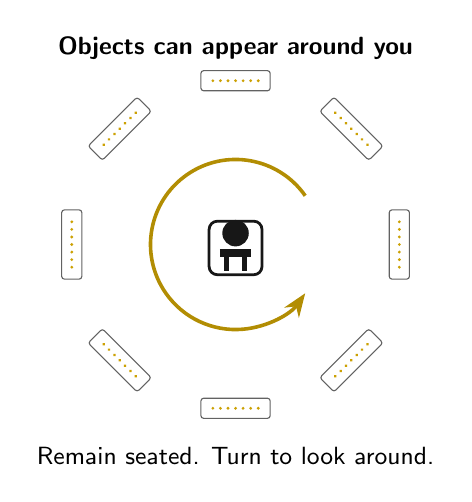
\begin{tikzpicture}[scale=0.8]
\foreach \a in {0,45,...,315}{
  \begin{scope}[shift={(\a:2.6)},rotate=\a-90]
  \draw[rounded corners=1pt,draw=Gray,fill=white] (-0.55,-0.16) rectangle (0.55,0.16);
  \foreach \x in {-0.36,-0.24,-0.12,0,0.12,0.24,0.36}{\fill[Gold!80!black] (\x,0) circle (0.025);}
  \end{scope}
}
\draw[Ink,line width=1pt,rounded corners=3pt] (-0.42,-0.48) rectangle (0.42,0.37);
\fill[Ink] (0,0.18) circle (0.21);
\draw[Ink,line width=3pt] (-0.25,-0.13)--(0.25,-0.13);
\draw[Ink,line width=2pt] (-0.14,-0.16)--(-0.14,-0.42) (0.14,-0.16)--(0.14,-0.42);
\draw[-{Stealth[length=3mm]},line width=1.3pt,Gold!70!black] (35:1.35) arc (35:325:1.35);
\node[font=\small,align=center] at (0,-3.35) {Remain seated. Turn to look around.};
\node[font=\small\bfseries] at (0,3.12) {Objects can appear around you};
\end{tikzpicture}

{\small\color{Gray}Schematic, not to scale. Illustrates seated rotation only.}
\end{center}
\say{SAY}{``The next rounds are practice, and are meant to simply get you familiar with the task.''}
\action{ACTION}{Allow the user to complete the object selection practice rounds.}
\say{ASK}{``Do you have any questions about the controls or task?''}
\say{SAY}{``When you are ready, we will begin the first task block.''}
\clearpage
\step{6 First task block}
\action{INTERNAL SETTINGS}{Practice | Real | 30 rounds}
\action{RESEARCHER SETTINGS}{Confirm the saved first voice and planned trial schedule. Keep object layout, selection method, guidance policy and the finalized prompt wording constant across voices.}
\say{SAY}{``We will now begin the first task block. Find each target as quickly and accurately as you comfortably can. Stay seated and use the same controller ray and trigger selection you practiced. Tell me if you need to pause.''}
\action{ACTION}{Start block; monitor safety.}
\say{AT COMPLETION SAY}{``That task block is complete. Please stop and lower your hands comfortably.''}
\say{SAY}{``These questions ask about your workload, your experience of the activity and the agent. There are no right answers. Please answer based on the block you just finished.''}
\action{ACTION}{Administer Survey Block \#1.}
\say{SAY}{``You may take a short break of up to 5 minutes. Tell me when you are ready to continue.''}
\say{BEFORE CONTINUING ASK}{``Do you feel comfortable and well enough to continue?''}
\step{Second Task Block}
\action{INTERNAL SETTINGS}{| Assigned condition | 30 valid attempts}
\action{INTERNAL SETTINGS}{READ ONLY THE ASSIGNED CONDITION SCRIPT:}
\say{SAY}{``We will now begin the second task block. The task and selection method are the same. Find each target as quickly and accurately as you comfortably can, and tell me if you need to pause.''}
\action{ACTION}{Start block; monitor safety.}
\say{AT COMPLETION SAY}{``The search task is complete. Please stop turning. We will finish the questions about this block, then I will help you remove the headset.''}
\say{SAY}{``These questions ask about your workload, your experience of the activity and the agent. There are no right answers. Please answer based on the block you just finished.''}
\action{ACTION}{Administer Survey Block \#2.}
\clearpage
\step{9 Final Qualtrics}
\say{SAY}{``Please complete the final questionnaire. It asks about your experiences with the two voices. It is fine to have no preference. We are interested in what you experienced, including anything distracting, uncomfortable or unhelpful.''}
\say{SAY}{``Some follow-up questions may appear depending on your answers and the timing condition you experienced. Answer based on your own experience and tell me when you have submitted it.''}
\action{EXPLORATORY FOLLOW-UP}{After open responses, ask ``Did either voice feel like your own thoughts, like another person helping, or neither?'' Record this as an exploratory report, not proof of an internal-dialogue mechanism.}
\action{ACTION}{Administer Post-Study Survey Block}
\step{10 Debrief and finish}
\say{SAY}{``Thank you. This study compares participant-preferred and self-similar voices during gaze-guided object search. Both voices provide gaze-contingent assistance. We are examining task performance and how participants experience the activity and assistant.''}
\say{SAY}{``Your data are stored under a coded participant ID. Please avoid discussing the timing condition or study details with people who may participate later, because knowing them in advance could affect their behavior.''}
\say{ASK}{``Do you have any questions about the study or your experience?''}
\say{SAY}{``Thank you for participating. We are finished.''}
\step{Immediate stop or pause criteria}
\meeting{PAUSE OR STOP}{Participant request, dizziness, nausea, headache, eye strain, fatigue, pain, distress, unsafe movement or equipment failure. Help the participant remain seated and remove the headset when needed.}

\clearpage
\step{Final researcher check}
{\color{ActionInk}\itshape
\begin{itemize}
\item {Confirm both block surveys and final interview/symptom records, or record why incomplete. }
\item {Match participant, run, block and voice identifiers.}
\item {Secure data and sanitize equipment.}
\end{itemize}
}
\step{Appendix Current recording passage}
\meeting{CURRENT RECORDING PASSAGE}{``Locate the red sphere. Look toward the upper shelf. Move your gaze slowly to the right. Check the blue cube near the center. Compare each object's color and shape. Scan the lower row from left to right. Look beside the purple cylinder. Point the controller ray at the target and check its highlight. Press the trigger to select the matching object. Take a short pause. Get ready for the next round.''}
\end{document}
